\cleardoublepage

\chapter{Algoritmos cuánticos}
\label{Cap3:Algoritmos}

El siguiente paso en este camino hacia la unión entre la computación cuántica y el \textit{testing} metamórfico es la creación de algoritmos o programas cuánticos que nos ayuden a resolver problemas propuestos o avanzar. \newline

Todo el desarrollo de estos algoritmos se pueden encontrar en los libros principales \cite{B:Nielsen:2002}\cite{B:QuantumScientist:2008}. Presentaremos a continuación todos los algoritmos finales que nos permiten obtener nuestros objetivos, si bien es cierto, solo vamos a presentar el camino completo de creación del algoritmo de Deutsch por su simplicidad. Esto se debe a que para alcanzar nuestro objetivo debemos ir haciendo modificaciones y cálculos sobre nuestros algoritmos hasta dar con la combinación correcta de puertas que nos permita resolverlo.\newline

Esta sección va a seguir prácticamente la misma estructura para cada apartado, a excepción de la suma. Empezará con una introducción, seguida de la exposición del problema a resolver. Entonces nos dispondremos a presentar el algoritmo que lo resuelve, o como lo creamos, y las pruebas realizadas. Es necesario recordar que toda la programación realizada sobre estos algoritmos se encuentra en el repositorio de GitHub \url{https://github.com/sinugarc/TFG.git}

\section{Suma}
\label{Sec3.1:Suma}
 Este primer algoritmo nos va a servir como primera toma de contacto con la programación cuántica, las puertas que podemos utilizar y el uso de \textit{Qiskit}. Veamos cual es el problema a resolver:\newline

 \textbf{Problema 1}: Dadas dos cadenas binarias de igual longitud, queremos obtener la suma bit a bit de ambas.\newline

 Esta operación se va a realizar posteriormente y se usará $\oplus$ como notación. La implementación de este problema es muy simple, bastará con incluir tantos bit ancilla como longitud tenga la cadena que almacene el resultado, así nos aseguramos que no se modifiquen los valores originales y bastará con utilizar la puerta $CNOT$ para ir modificando los valores ancilla correspondientes. Dando lugar en los valores ancilla al resultado de la suma bit a bit de ambas cadenas.\newline

 (PONER CIRCUITO)

 \textbf{Problema 2}: Dadas dos cadenas binarias, queremos obtener la suma de ambas, como si estas fueran representación de número naturales.\newline

 (EXPLICAR Y PONER EL PRIMER CIRCUITO PROGRAMADO)

\section{Deutsch}
\label{Sec3.2:Deutsch}

 El algoritmo de Deutsch\cite{B:QuantumScientist:2008} fue propuesto por David Deutsch en 1985, siendo este uno de los primeros algoritmos propuestos y en sí, el que se podría entender como uno de los problema más simples. Sea $f:\{0,1\}\rightarrow\{0,1\}$, diremos que $f$ es \textbf{balanceada} si $f(0)\neq f(1)$ y diremos que es \textbf{constante} si $f(0)=f(1)$. \newline

 \textbf{Problema}: Dada una función $f:\{0,1\}\rightarrow\{0,1\}$ balanceada o constante, la cual no podemos observar su definición. Queremos determinar si esta función es constante o balanceada.\newline

 \textbf{Solución clásica}: Tenemos que evaluar $f$ en ambos valores y comparar las soluciones.\newline

 Veamos ahora que podemos hacer con un ordenador cuántico, ¿seremos capaces de evaluar $f$ una única vez? \newline

 Primero observamos un ejemplo particular y cómo vamos a llevarlo a un circuito cuántico. Sea $f(0)=1$ y $f(1)=0$, buscamos una matriz unitaria que nos permita representarla en un circuito cuántico, aunque tendremos que hacer alguna modificación más. Por ahora lo que obtenemos es,

 \begin{equation*}
     \begin{matrix}
           & \begin{matrix} \textbf{0} & \textbf{1} \end{matrix} \\
         \begin{matrix} \textbf{0} \\ \textbf{1} \end{matrix} & \begin{bmatrix}
             0 & 1 \\
             1 & 0
         \end{bmatrix}
     \end{matrix}
 \end{equation*}

 \vspace{5pt}

 Donde la columna representa la entrada y la fila la salida. Como ya se mencionó al explicar los qubits del circuito (figura 2.2), es importante conservar la entrada y por lo tanto si $U_{f}$ es la caja negra que representa a $f$, nuestro circuito será:

 \vspace{10pt}

 \begin{center}$\Qcircuit @C=1em @R=.7em {\lstick{|x\rangle}&  \multigate{1}{U_{f}} &\qw & \rstick{|x\rangle}\\ \lstick{|y\rangle} &\ghost{U_{f}} & \qw & \rstick{|y \oplus f(x)\rangle}}$ \end{center}

 \vspace{7pt}

 Es más, si aplicáramos $U_{f}$ dos veces obtendríamos la entrada:

 \vspace{10pt}

 \begin{center}$\Qcircuit @C=1em @R=.7em {\lstick{|x\rangle} & \multigate{1}{U_{f}} & \qw & \qw & \ustick{|x\rangle} \qw & \qw & \qw & \multigate{1}{U_{f}} & \qw & \rstick{|x\rangle}\\ \lstick{|y\rangle} & \ghost{U_{f}} & \qw & \qw & \dstick{|y \oplus f(x)\rangle} \qw & \qw & \qw &\ghost{U_{f}} & \qw & \rstick{|y\rangle}}$\end{center}

 \vspace{14pt}

 Esto se debe a que $f(x)\oplus f(x) = 0$. Pero claro, ¿qué matriz realmente representa a $U_{f}$? Veamos como quedaría respecto a la base:

 \vspace{5pt}
 \begin{center}
 \begin{blockarray}{ccccc}
         & $\mathbf{|00\rangle}$ & $\mathbf{|01\rangle}$ & $\mathbf{|10\rangle}$ & $\mathbf{|11\rangle}$\\
    \begin{block}{c[cccc]}
        $\mathbf{|00\rangle}$ & 0 & 1 & 0 & 0 \\
        $\mathbf{|01\rangle}$ & 1 & 0 & 0 & 0 \\
        $\mathbf{|10\rangle}$ & 0 & 0 & 1 & 0 \\
        $\mathbf{|11\rangle}$ & 0 & 0 & 0 & 1
     \end{block}
\end{blockarray}
\end{center}

\vspace{5pt}

Se podría comprobar que esta matriz es su propia adjunta, por lo que es invertible y unitaria. Por lo que cumple las características necesarias para ser una puerta de un circuito cuántico.\newline

 Ahora que ya tenemos la caja negra deseada, determinada por una matriz unitaria, nos queremos poner a resolver el problema. Como comenté en la introducción de este capítulo, esta va a ser el único algoritmo al que le vamos a seguir la pista de razonamiento de principio a final, es decir, partiremos de una idea inicial y acabaremos en el algoritmo de Deutsch que resuelve este problema.\newline

 Nuestro objetivo es mejorar la complejidad de la solución del problema respecto a la solución clásica. Recordamos que necesitamos evaluar $f$ dos veces, por lo que nuestro objetivo va a ser obtener el resultado evaluando $f$ una única vez. Para ello nos vamos a sustentar en la superposición, para así analizar que ocurre en el $|0\rangle$ y en el $|1\rangle$ al mismo tiempo, es decir, vamos a tener que utilizar la puerta de Hadamard. \newline
 
 \textbf{Primer intento}: Tomamos nuestro primer \textit{input} para el problema, por ejemplo $|x\rangle=|0\rangle$ e $|y\rangle=|0\rangle$ y creamos el primer circuito:

 \vspace{5pt}

 \begin{center}$\Qcircuit @C=1.5em @R=.7em {\lstick{|0\rangle} & \qw & \gate{H} & \qw &\multigate{1}{U_{f}} & \qw & \qw & \qw  \\ \lstick{|0\rangle} & \dstick{\begin{matrix} \Uparrow \\ |\varphi_{0}\rangle \end{matrix}} \qw & \qw  & \dstick{\begin{matrix} \Uparrow \\ |\varphi_{1}\rangle \end{matrix}} \qw & \ghost{U_{f}} & \dstick{\begin{matrix} \Uparrow \\ |\varphi_{2}\rangle \end{matrix}} \qw & \meter & \qw \\}$\end{center}

\vspace{30pt}

Donde cada $\varphi_{i}$ va a representar el estado del sistema en cada momento, esto nos va a ayudar a analizar de forma determinista lo que ocurre en nuestro circuito.\newline

Podemos resumir el circuito como  $U_{f}(H\otimesI)|0,0\rangle$, veamos ahora que estados tenemos en cada instante $i$:

\begin{itemize}
    \item $\mathbf{|\varphi_{0}\rangle} = |0\rangle \otimes |0\rangle = |0,0\rangle$

    \item $\mathbf{|\varphi_{1}\rangle} = (H\otimes I)|0,0\rangle = \left[ \dfrac{|0\rangle + |1\rangle}{\sqrt{2}}\right] |0\rangle = \dfrac{|0,0\rangle+|1,0\rangle}{\sqrt{2}}$

    \item  $\mathbf{|\varphi_{2}\rangle} = \dfrac{|0,f(0)\rangle+|1,f(1)\rangle}{\sqrt{2}}$
\end{itemize}

Si nos fijamos en el ejemplo que expuesto al principio del algoritmo obtendríamos el siguiente estado antes de la medición:

\begin{equation}
    |\varphi_{2}\rangle=\begin{bmatrix}
        0 & 1 & 0 & 0 \\
        1 & 0 & 0 & 0 \\
        0 & 0 & 1 & 0 \\
        0 & 0 & 0 & 1
    \end{bmatrix}
    \begin{bmatrix}
        \frac{1}{\sqrt{2}} \\ 0 \\ \frac{1}{\sqrt{2}} \\ 0 
    \end{bmatrix} = 
    \begin{bmatrix}
        0 \\ \frac{1}{\sqrt{2}} \\ \frac{1}{\sqrt{2}} \\ 0 
    \end{bmatrix} = \dfrac{|0,1\rangle + |1,0\rangle}{\sqrt{2}}
\end{equation}

De aquí podemos observar, que sin importar donde hagamos la medición, el resultado no va a ser concluyente, porque vamos a tener una probabilidad de 0.5 de obtener $|0\rangle$ o $|1\rangle$. Es decir, este primer intento no nos sirve para nuestro objetivo. \newline

\textbf{Segundo intento}: Veamos ahora que ocurre si en vez de poner en superposición el primer qubit, ahora ponemos el segundo, tomando $|1\rangle$ como \textit{input}:

 \vspace{5pt}

 \begin{center}$\Qcircuit @C=1.5em @R=.7em {\lstick{|x\rangle} & \qw & \qw & \qw &\multigate{1}{U_{f}} & \qw & \qw & \qw  \\ \lstick{|1\rangle} & \dstick{\begin{matrix} \Uparrow \\ |\varphi_{0}\rangle \end{matrix}} \qw & \gate{H}  & \dstick{\begin{matrix} \Uparrow \\ |\varphi_{1}\rangle \end{matrix}} \qw & \ghost{U_{f}} & \dstick{\begin{matrix} \Uparrow \\ |\varphi_{2}\rangle \end{matrix}} \qw & \meter & \qw \\}$\end{center}

\vspace{30pt}

Ahora iremos directamente a $|\varphi_{2}\rangle$ :

\begin{equation}
    |\varphi_{2}\rangle=|x\rangle \left[ \dfrac{|0\otimes f(x)\rangle - |1\otimes f(x)\rangle}{\sqrt{2}} \right] = \begin{cases} |x\rangle \:  \left[ \dfrac{|0\rangle-|1\rangle}{\sqrt{2}}\right] \;\; si \: f(x) = 0 \\ \\ |x\rangle \: \left[ \dfrac{|0\rangle-|1\rangle}{\sqrt{2}} \right] \;\; si \: f(x) = 1 \end{cases}
\end{equation}\newline

Esto lo podemo resumir como:

\begin{equation}
    |\varphi_{2}\rangle = (-1)^{f(x)} \;|x\rangle \; \left[ \dfrac{|0\rangle-|1\rangle}{\sqrt{2}}\right]
\end{equation}\newline

Pero al igual que en intento anterior, al intentar medir en cualquiera de ambos qubits no obtendríamos ningún resultado concluyente. Esto nos va a llevar al último intento.\newline

\textbf{Tercer intento}, \textbf{Algoritmo de Deutsch}: Al no ser capaces de obtener un resultado poniendo sólo un qubit en superposición, esta vez vamos a poner ambos en estado de superposición, con  el \textit{input} $|0,1\rangle$. Además, vamos a medir sobre el qubit superior tras aplicar una puerta de Hadamard, que recordamos es su propia inversa. Este es el circuito final que representa al algoritmo de Deutsch:

 \vspace{5pt}

 \begin{center}$\Qcircuit @C=1.5em @R=.7em {\lstick{|0\rangle} & \qw & \gate{H} & \qw &\multigate{1}{U_{f}} & \qw & \gate{H} & \qw & \meter & \qw  \\ \lstick{|1\rangle} & \dstick{\begin{matrix} \Uparrow \\ |\varphi_{0}\rangle \end{matrix}} \qw & \gate{H}  & \dstick{\begin{matrix} \Uparrow \\ |\varphi_{1}\rangle \end{matrix}} \qw & \ghost{U_{f}} & \dstick{\begin{matrix} \Uparrow \\ |\varphi_{2}\rangle \end{matrix}} \qw & \qw & \dstick{\begin{matrix} \Uparrow \\ |\varphi_{3}\rangle \end{matrix}} \qw & \qw & \qw }$\end{center}

\vspace{30pt}

Esto matricialmente nos queda como $(H\otimes I)\:U_{f}\:(H\otimes H)\:|0,1\rangle$ .\newline

Analizamos ahora todos los estados $|\varphi_{i}\rangle$:

\begin{itemize}
    \item $\mathbf{|\varphi_{0}\rangle} = |0\rangle \otimes |1\rangle = |0,1\rangle$

    \vspace{5pt}

    \item  $\mathbf{|\varphi_{1}\rangle} = \left[ \dfrac{|0\rangle + |1\rangle}{\sqrt{2}}\right] \left[ \dfrac{|0\rangle - |1\rangle}{\sqrt{2}}\right]$

    \vspace{5pt}

    \item $\mathbf{|\varphi_{2}\rangle} = \left[ \dfrac{(-1)^{f(0)}\:|0\rangle + (-1)^{f(1)}\:|1\rangle}{\sqrt{2}}\right] \left[ \dfrac{|0\rangle - |1\rangle}{\sqrt{2}}\right]$\newline 
    
    Hemos obtenido este resultado substituyendo $|x\rangle$ en el la ecuación 3.3 (link). Pero veamos que ocurre separando $(-1)^{f(0)}\:|0\rangle + (-1)^{f(1)}\:|1\rangle$ según nuestras posibilidades:
    \begin{itemize}
        \item $f$ es constante: $\dfrac{(-1)^{f(0)}\:|0\rangle + (-1)^{f(1)}\:|1\rangle}{\sqrt{2}} = (\pm 1)\left[ \dfrac{|0\rangle - |1\rangle}{\sqrt{2}}\right]$

        \vspace{5pt}
        
        \item $f$ es balanceada: $\dfrac{(-1)^{f(0)}\:|0\rangle + (-1)^{f(1)}\:|1\rangle}{\sqrt{2}} = (\pm 1)\left[ \dfrac{|0\rangle + |1\rangle}{\sqrt{2}}\right]$

    \end{itemize}

    \vspace{5pt}
    
    \item Y por último obtenemos:
    \begin{equation}\mathbf{|\varphi_{3}\rangle} = \begin{cases} (\pm 1)\:|0\rangle \left[ \dfrac{|0\rangle - |1\rangle}{\sqrt{2}}\right] \;\; si \: f(x)\:\text{es constante} \\ \\ (\pm 1)\:|1\rangle \left[ \dfrac{|0\rangle - |1\rangle}{\sqrt{2}}\right] \;\; si \: f(x)\:\text{es balanceada} \end{cases}\end{equation}
\end{itemize}

Por lo que hemos conseguido nuestro objetivo. Tras una única evaluación de $f$ según la medición del primer qubit, sabremos si $f$ es constante con medición $|0\rangle$ o balanceada, $|1\rangle$. Consiguiendo así nuestro objetivo.\newline

\section{Deutsch-Jozsa}
\label{Sec3.3:Deutsch-Jozsa}
 El algoritmo de Deutsch-Jozsa\cite{B:QuantumScientist:2008} es una generalización del algoritmo de Deutsch del apartado anterior, pero ahora trabajamos con $f:\{0,1\}^{n} \rightarrow\{0,1\}$. El domino se puede entender como los números escrito en binario de 0 a $2^{n}-1$. En este caso vamos a redefinir los conceptos anteriores:

 \begin{itemize}
     \item Diremos que $f$ es \textbf{constante} si todo el domino va a 0 ó a 1.
     \item Diremos que $f$ es \textbf{balanceada} si exactamente la mitad del domino va a 0 y la otra mitad va a 1.
 \end{itemize}

 \textbf{Problema}\label{P:DJ}: Dada una función $f:\{0,1\}^{n} \rightarrow\{0,1\}$ balanceada o constante, la cual no podemos observar su definición. Queremos determinar si esta función es constante o balanceada.\newline

 \textbf{Solución clásica}: Vamos a tener que evaluar la función $f$ tantas veces como sea necesario. El mejor caso es tras 2 ejecuciones, ya que puede darse la situación en la que es balanceada y cada ejecución da un resultado diferente. Por otra parte, el peor caso se da con $2^{n-1}+1$ ejecuciones, ya que si las primeras $2^{n-1}$ son iguales, la siguiente nos va a determinar si es constante o balanceada. Todo esto se debe a que como hipótesis tenemos que es una de las 2 cosas. \newline

 Vamos a partir del circuito inicial, donde $U_{f}$ determina la función $f$:

 \vspace{10pt}

 \begin{center}$\Qcircuit @C=1.5em @R=1em {\lstick{|\mathbf{x}\rangle}& \qw {/^{n}} & \multigate{1}{U_{f}} & \qw {/^{n}} &\qw & \rstick{|\mathbf{x}\rangle}\\ \lstick{|y\rangle} & \qw &\ghost{U_{f}} & \qw & \qw & \rstick{|y \oplus f(\mathbf{x})\rangle}}$ \end{center}

 \vspace{7pt}

 Hay que destacar que $|\mathbf{x}\rangle=|x_{0}x_{1}...x_{n-1}\rangle$, por eso posteriormente escribimos $/^{n}$, para indicar que son n qubits.\newline

 \textbf{Algoritmo de Deutsch-Jozsa\label{A:DJ}}:

 \vspace{10pt}

 \begin{center}$\Qcircuit @C=1.5em @R=1em {
 \lstick{|\mathbf{0}\rangle}& \qw {/^{n}} & \gate{H^{\otimes n}} & \qw {/^{n}} & \multigate{1}{U_{f}} & \qw {/^{n}} & \gate{H^{\otimes n}} & \qw {/^{n}} & \meter & \qw \\ \lstick{|1\rangle} & \dstick{\begin{matrix} \Uparrow \\ |\varphi_{0}\rangle \end{matrix}} \qw & \gate{H} & \dstick{\begin{matrix} \Uparrow \\ |\varphi_{1}\rangle \end{matrix}} \qw &\ghost{U_{f}} & \dstick{\begin{matrix} \Uparrow \\ |\varphi_{2}\rangle \end{matrix}} \qw & \qw & \dstick{\begin{matrix} \Uparrow \\ |\varphi_{3}\rangle \end{matrix}} \qw  & \qw & \qw}$ \end{center}

 \vspace{30pt}

 Que en término de matrices es: $(H^{\otimes n} \otimes I)\:U_{f}\:(H^{\otimes n} \otimes H)\:|\mathbf{0},1\rangle$ \newline

 Antes de analizar los estados en cada $|\varphi_{i}\rangle$, vamos a estudiar que ocurre cuando tenemos la puerta $H^{\otimes n}$ y como se comporta sobre los diferentes estados, así como la notación que utilizamos, ya que esta será necesaria en el análisis de los $|\varphi_{i}\rangle$. \newline

 El estudio sobre las características de $H^{\otimes n}$ se pueden estudiar en profundidad en \citealp[\textit{Quantum computing for computer scientists}]{B:QuantumScientist:2008}, aquí resumiremos los resultados principales que nos van a permitir profundizar en los circuitos cuánticos, ya que la aplicación de esta puerta es muy común.\newline

 Antes de meternos en $H^{\otimes n}$, vamos a definir un producto interno en $\mathbb{Z}_{2}$:\newline

 \begin{equation*}
     \langle\:,\:\rangle\::\{0,1\}^{n} \times \{0,1\}^{n} \rightarrow \{0,1\}\end{equation*}

 Si $\mathbf{x}=x_{0}x_{1}...x_{n-1}$ e $\mathbf{y}=y_{0}y_{1}...y_{n-1}$, entonces:

 \begin{equation*}
     \begin{split}
     \langle\mathbf{x},\mathbf{y}\rangle &= \langle x_{0}x_{1}...x_{n-1},y_{0}y_{1}...y_{n-1}\rangle \\ &= (x_{0}\land y_{0})\oplus(x_{1}\land y_{1})\oplus...\oplus(x_{n-1}\land y_{n-1}) \\ &= x_{0}y_{0}\oplus x_{1}y_{1}\oplus ... \oplus x_{n-1}y_{n-1}
     \end{split}
 \end{equation*}

 Donde $\land$ es la operación lógica AND y $\oplus$ la operación lógica XOR.\newline

 También definimos, $\mathbf{x}\oplus\mathbf{y}=x_{0}\oplus y_{0},x_{1}\oplus y_{1},...,x_{n-1}\oplus y_{n-1}$ como la suma binaria bit a bit.\newline

 Con esto obtenemos las siguiente propiedades del producto interno:

 \begin{itemize}
     \item $\langle \mathbf{x} \oplus \mathbf{x}',\mathbf{y}\rangle=\langle \mathbf{x},\mathbf{y}\rangle \oplus \langle \mathbf{x}',\mathbf{y}\rangle$

     \item $\langle \mathbf{x},\mathbf{y} \oplus \mathbf{y}'\rangle=\langle \mathbf{x},\mathbf{y}\rangle \oplus \langle \mathbf{x},\mathbf{y}'\rangle$

     \item $\langle 0\cdot \mathbf{x},\mathbf{y}\rangle=\langle\mathbf{0},\mathbf{y}\rangle=0$

     \item $\langle \mathbf{x}, 0 \cdot \mathbf{y}\rangle=\langle \mathbf{x},\mathbf{0}\rangle=0$
 \end{itemize}

 Una vez definidas estas operaciones y propiedades vamos a poder definir la matriz que caracteriza a $H^{\otimes n}$. Cabe recordar que cada fila y cada columna representa un elemento de la base, que se corresponde con la representación binaria de la fila y la columna desde 0:
 
 \begin{equation}H^{\otimes n} [\mathbf{i},\mathbf{j}] = \dfrac{1}{\sqrt{2^{n}}}(-1)^{\langle\mathbf{i},\mathbf{j}\rangle}\end{equation}

 Desde aquí podemos obtener las 2 expresiones que utilizaremos a continuación:

 \begin{equation}
     H^{\otimes n}|\mathbf{0}\rangle=H^{\otimes n}[-,\mathbf{0}]=\dfrac{1}{\sqrt{2^{n}}}\sum_{\mathbf{x} \in \{0,1\}^{n}} |\mathbf{x}\rangle
 \end{equation}

 \begin{equation}
     H^{\otimes n}|\mathbf{y}\rangle=H^{\otimes n}[-,\mathbf{y}]=\dfrac{1}{\sqrt{2^{n}}}\sum_{\mathbf{x} \in \{0,1\}^{n}} (-1)^{\langle\mathbf{x},\mathbf{y}\rangle}|\mathbf{x}\rangle
 \end{equation}
 
 Ahora ya si que vamos a observar los estados que se producen en los distintos momentos del circuito:

 \begin{itemize}
     \item $\mathbf{|\varphi_{0}\rangle} = |\mathbf{0},1\rangle$

    \vspace{5pt}

    \item  $\mathbf{|\varphi_{1}\rangle} = \left[ \dfrac{\sum_{\mathbf{x} \in \{0,1\}^{n}}|\mathbf{x}\rangle}{\sqrt{2^{n}}}\right] \left[ \dfrac{|0\rangle - |1\rangle}{\sqrt{2}}\right]$

    \vspace{5pt}

    \item $\mathbf{|\varphi_{2}\rangle} =\left[ \dfrac{\sum_{\mathbf{x} \in \{0,1\}^{n}}(-1)^{f(\mathbf{x})}|\mathbf{x}\rangle}{\sqrt{2^{n}}}\right] \left[ \dfrac{|0\rangle - |1\rangle}{\sqrt{2}}\right]$

    \vspace{5pt}

    \item Ahora tenemos que superponer la superposición, pero en este caso no es la inversa ya que se aplica sobre otros estados $|\mathbf{z}\rangle$:

    \begin{equation}
        \begin{split}\mathbf{|\varphi_{3}\rangle} &= \left[ \dfrac{\sum_{\mathbf{x} \in \{0,1\}^{n}}(-1)^{f(\mathbf{x})}\sum_{\mathbf{z} \in \{0,1\}^{n}}(-1)^{\langle\mathbf{z},\mathbf{x}\rangle}|\mathbf{z}\rangle}{2^{n}}\right] \left[ \dfrac{|0\rangle - |1\rangle}{2^{n}}\right] \\ &= \left[ \dfrac{\sum_{\mathbf{x} \in \{0,1\}^{n}}\sum_{\mathbf{z} \in \{0,1\}^{n}}(-1)^{f(\mathbf{x})}(-1)^{\langle\mathbf{z},\mathbf{x}\rangle}|\mathbf{z}\rangle}{2^{n}}\right] \left[ \dfrac{|0\rangle - |1\rangle}{2^{n}}\right] \\ &= \left[ \dfrac{\sum_{\mathbf{x} \in \{0,1\}^{n}}\sum_{\mathbf{z} \in \{0,1\}^{n}}(-1)^{f(\mathbf{x})\oplus\langle\mathbf{z},\mathbf{x}\rangle}|\mathbf{z}\rangle}{2^{n}}\right] \left[ \dfrac{|0\rangle - |1\rangle}{2^{n}}\right]
        \end{split}
    \end{equation}
 \end{itemize}

 El último paso a analizar y que nos determinará la validez o el que esperamos de este algoritmo es al medición de los primeros n-qubits. Otra manera de estudiar la medición es directamente preguntarnos cual es la probabilidad de que $|\varphi_{3}\rangle$ colapse a $|\mathbf{0}\rangle$ al realizar la medición. Esto es análogo a si bien en el algoritmo anterior nos interesaba medir cuando $|\mathbf{z}\rangle=|\mathbf{0}\rangle$, que por las propiedades estudiadas anteriormente $\langle\mathbf{z},\mathbf{x}\rangle=\langle\mathbf{0},\mathbf{x}\rangle=0$. Con este resultado, si volvemos a la ecuación 3.5 (link):

 \begin{equation}
     \mathbf{|\varphi_{3}\rangle}=\left[ \dfrac{\sum_{\mathbf{x} \in \{0,1\}^{n}}(-1)^{f(\mathbf{x})}|\mathbf{0}\rangle}{2^{n}}\right] \left[ \dfrac{|0\rangle - |1\rangle}{\sqrt{2}}\right]
 \end{equation}

 Veamos cual sería el estado del primer qubit dependiendo de de nuestras posibilidades:

 \begin{itemize}
     \item $f$ es constante:  $\dfrac{\sum_{\mathbf{x} \in \{0,1\}^{n}}(-1)^{f(\mathbf{x})}|\mathbf{0}\rangle}{2^{n}}=\dfrac{\sum_{\mathbf{x} \in \{0,1\}^{n}}(-1)^{f(\mathbf{x})}|\mathbf{0}\rangle}{2^{n}}=\dfrac{(\pm1)2^{n}|\mathbf{0}\rangle}{2^{n}}=(\pm1)|\mathbf{0}\rangle$

     \item $f$ es balanceada: 
     $\dfrac{\sum_{\mathbf{x} \in \{0,1\}^{n}}(-1)^{f(\mathbf{x})}|\mathbf{0}\rangle}{2^{n}}=\dfrac{0|\mathbf{0}\rangle}{2^{n}}=0|\mathbf{0}\rangle$
 \end{itemize}

 Por lo que podemos concluir que este algoritmo resuelve nuestro problema con una única evaluación de $f$. Si el resultado es $|\mathbf{0}\rangle$, $f$ es constante y si es otro cualquiera, $f$ es balanceada. \newline

 \textbf{Observación}: Hay que tener en cuenta, que si la función no es ni balanceada ni constante, este algoritmo no soluciona el problema y los resultados no son concluyentes. Esto se debe a que cualquier valor que nos devuelva el algoritmo tiene un interpretación $|\textbf{0}\rangle$ $f$ constante y si no, $f$ es balanceada. Es decir, si tenemos una función $f$ que no es ni constante ni balanceada, el resultado sea el que sea va a ser erróneo. Y esto explica porque es una de nuestras hipótesis. \newline

\textbf{Oráculo}: El oráculo que utilizamos para este algoritmo puede venir de dos sitios distintos. Podemos programarlo con ayuda de qiskit\footnote{\url{https://learn.qiskit.org/course/ch-algorithms/deutsch-jozsa-algorithm}}, ya que nos explica como crear el oráculo de DJ, sea la función balanceada o constante. O bien, una vez definida la función crear la matriz que representa al operador.\newline
 
\textbf{Simulaciones}: En el repositorio podemos encontrar este algoritmo programado con ayuda de \textit{Qiskit}. Una de las peculiaridades que encontramos es la forma en la que \textit{Qiskit} nos presenta los qubits, más bien hay una permutación en la base respecto a la generalmente utilizamos al formalizar matrices. Esto puede ser un problema cuando las puertas las creamos como un operador a partir de la matriz que las determina. El ejemplo de esta situación esta programado (en el test del repositorio), así como pruebas del algoritmo de DJ con la misma matriz. \newline

Si bien es cierto que todos aquellos algoritmos que tiene programado el oráculo con el procedimiento de Qiskit de forma balanceada su resultado es el ket $|\mathbf{1}\rangle$, esto no tiene porque ser cierto. Si recordamos el análisis final del algoritmo, si obtenemos $|\textbf{0}\rangle$ entonces $f$ es constante y si no, $f$ es balanceada. Por lo que si miramos el algoritmo programado con un operador matricial, podemos observar como el resultado no es ni $|\textbf{0}\rangle$, ni $|\textbf{1}\rangle$, si no que obtenemos $|01\rangle$.


\section{Bernstein-Vazirani}
\label{Sec3.4:BV}

El algoritmo de Bernstein-Vazirani, fué presentado por Ethan Bernstein and Umesh Vazirani\cite{AR:BV:1997}. Se puede entender que este algoritmo es una generalización más del algoritmo de Deutsch-Jozsa \footnote{https://learn.qiskit.org/course/ch-algorithms/bernstein-vazirani-algorithm}. \newline

\textbf{Problema}: Sea $f:\{0,1\}^{n} \rightarrow \{0,1\}$, sea $\mathbf{s}=s_{0}s_{1}...s_{n-1}$, por hipótesis $f(\mathbf{x})=\mathbf{s}\cdot \mathbf{x}\: \text{mod}\:2 = s_{0}x_{0} \oplus s_{1}x_{1} \oplus ... \oplus s_{n-1}x_{n-1}$. Queremos obtener la cadena $\mathbf{s}$.\newline

\textbf{Solución clásica}: Ejecutamos la función $f$ $n$ veces una con cada elemento de la base canónica. Esto nos permitirá obtener los $n$ elementos de $\mathbf{s}$.\newline

\textbf{Algoritmo de Bernstein-Vazirani}:

 \vspace{10pt}

 \begin{center}$\Qcircuit @C=1.5em @R=1em {
 \lstick{|\mathbf{0}\rangle}& \qw {/^{n}} & \gate{H^{\otimes n}} & \qw  & \qw {/^{n}} & \multigate{1}{U_{f}} & \qw {/^{n}} & \gate{H^{\otimes n}} & \qw {/^{n}} & \meter & \qw \\ \lstick{|0\rangle} & \dstick{\begin{matrix} \Uparrow \\ |\varphi_{0}\rangle \end{matrix}} \qw & \gate{H} & \gate{Z} & \dstick{\begin{matrix} \Uparrow \\ |\varphi_{1}\rangle \end{matrix}} \qw &\ghost{U_{f}} & \dstick{\begin{matrix} \Uparrow \\ |\varphi_{2}\rangle \end{matrix}} \qw & \qw & \dstick{\begin{matrix} \Uparrow \\ |\varphi_{3}\rangle \end{matrix}} \qw  & \qw & \qw}$ \end{center}

 \vspace{30pt}

 De forma matricial: $(H^{\otimes n} \otimes I)\: U_{f}\:(I\otimes Z)\:(H^{\otimes n} \otimes H) |\mathbf{0},0\rangle$ \newline

 Veamos ahora los estados alcanzados, similares al circuito anterior:

 \begin{itemize}
     \item $\mathbf{|\varphi_{0}\rangle} = |\mathbf{0},0\rangle$

    \vspace{5pt}

    \item  $\mathbf{|\varphi_{1}\rangle} = \left[ \dfrac{\sum_{\mathbf{x} \in \{0,1\}^{n}}|\mathbf{x}\rangle}{\sqrt{2^{n}}}\right] \left[ \dfrac{|0\rangle - |1\rangle}{\sqrt{2}}\right]$

    \vspace{5pt}

    \item Aplicamos las función $f$:
    
    \begin{equation} \label{eq:BV:phi2}
    \mathbf{|\varphi_{2}\rangle} =\left[ \dfrac{\sum_{\mathbf{x} \in \{0,1\}^{n}}(-1)^{f(\mathbf{x})}|\mathbf{x}\rangle}{\sqrt{2^{n}}}\right] \left[ \dfrac{|0\rangle - |1\rangle}{\sqrt{2}}\right]\end{equation}

    \vspace{5pt}

    \item Ahora tenemos que superponer la superposición, aplicada sobre otros estados $|\mathbf{z}\rangle$:

    \begin{equation}\label{eq:BV:phi3}
        \begin{split}\mathbf{|\varphi_{3}\rangle} &= \left[ \dfrac{\sum_{\mathbf{x} \in \{0,1\}^{n}}(-1)^{f(\mathbf{x})}\sum_{\mathbf{z} \in \{0,1\}^{n}}(-1)^{\langle\mathbf{z},\mathbf{x}\rangle}|\mathbf{z}\rangle}{2^{n}}\right] \left[ \dfrac{|0\rangle - |1\rangle}{2^{n}}\right] \\ &= \left[ \dfrac{\sum_{\mathbf{x} \in \{0,1\}^{n}}\sum_{\mathbf{z} \in \{0,1\}^{n}}(-1)^{f(\mathbf{x})}(-1)^{\langle\mathbf{z},\mathbf{x}\rangle}|\mathbf{z}\rangle}{2^{n}}\right] \left[ \dfrac{|0\rangle - |1\rangle}{2^{n}}\right] \\ &= \left[ \dfrac{\sum_{\mathbf{x} \in \{0,1\}^{n}}\sum_{\mathbf{z} \in \{0,1\}^{n}}(-1)^{f(\mathbf{x})\oplus\langle\mathbf{z},\mathbf{x}\rangle}|\mathbf{z}\rangle}{2^{n}}\right] \left[ \dfrac{|0\rangle - |1\rangle}{2^{n}}\right] \\  &= \left[ \dfrac{\sum_{\mathbf{x} \in \{0,1\}^{n}}\sum_{\mathbf{z} \in \{0,1\}^{n}}(-1)^{\langle\mathbf{s},\mathbf{x}\rangle\oplus\langle\mathbf{z},\mathbf{x}\rangle}|\mathbf{z}\rangle}{2^{n}}\right] \left[ \dfrac{|0\rangle - |1\rangle}{2^{n}}\right] \\ &= \left[ \dfrac{\sum_{\mathbf{x} \in \{0,1\}^{n}}\sum_{\mathbf{z} \in \{0,1\}^{n}}(-1)^{\langle\mathbf{s}\oplus \mathbf{z},\mathbf{x}\rangle}|\mathbf{z}\rangle}{2^{n}}\right] \left[ \dfrac{|0\rangle - |1\rangle}{2^{n}}\right] \\
        \end{split}
    \end{equation}
 \end{itemize}

 Veamos que esta ocurriendo en ese primer bloque de qubits, que será al que apliquemos la medición, si bien en el algoritmo anterior nos interesaba medir cuando $|\mathbf{z}\rangle=|\mathbf{0}\rangle$, pero ahora queremos obtener la cadena $\mathbf{s}$, por lo que vamos a ver que sucede cuando $|\mathbf{z}\rangle=|\mathbf{s}\rangle$.

 \begin{equation}
    \dfrac{\sum_{\mathbf{x} \in \{0,1\}^{n}}(-1)^{\langle\mathbf{s}\oplus \mathbf{s},\mathbf{x}\rangle}|\mathbf{s}\rangle}{2^{n}} = \dfrac{\sum_{\mathbf{x} \in \{0,1\}^{n}}(-1)^{\langle\mathbf{0},\mathbf{x}\rangle}|\mathbf{s}\rangle}{2^{n}}= \dfrac{\sum_{\mathbf{x} \in \{0,1\}^{n}}|\mathbf{s}\rangle}{2^{n}} = |\mathbf{s}\rangle
 \end{equation}

 \vspace{5pt}

 ¿Qué está ocurriendo aquí?, lo que hemos observado es que la amplitud de $|\mathbf{s}\rangle$ es 1, y si recordamos la teoría de los sistemas cuánticos, la suma de los cuadrados de las amplitudes es 1. Es decir, las amplitudes del resto de posibles valores de $|\mathbf{z}\rangle$ es 0. Por lo que al hacer la medición sobre el primer bloque de qubits nos devolverá la cadena $\mathbf{s}$ deseada, al ser su probabilidad de aparición 1. Podemos concluir entonces que hemos obtenido la cadena $\mathbf{s}$ con una única ejecución de $f$, mejorando así la solución clásica para este algoritmo.\newline

 
 \textbf{Oráculo}: Antes de presentar las simulaciones realizadas, vamos a estudiar como a partir de una cadena $\mathbf{s}$ podemos construir un oráculo funcione como $f_{s}$. Según el valor en la cadena se ejecuta una puerta y otra. Sí el valor es 0, entonces pondremos una puerta identidad en la linea del qubit de esa posición para indicar que no se hace nada y si el valor es 1, pondremos una puerta CNOT entre el qubit de la posición y el qubit ancilla, donde el qubit de control es el de la posición del valor. Estos ejemplo se pueden encontrar en el archivo de BV sin puertas, la función \textit{$bv\_fgenerator(qc,n0,s)$}, veamos un par de ejemplos ahora:
 
 \begin{figure}[H]
    \centering
    \begin{subfigure}[H]{0.35\textwidth}
        \centering
        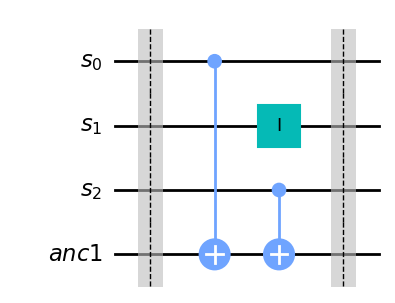
\includegraphics[width=\textwidth]{TFG/imagenes/BVgate1.png}
        \caption{Oráculo para la cadena $\mathbf{s}=101$}
        \label{sFig:BVgate1}
    \end{subfigure}
    \hspace{10pt}
    \begin{subfigure}[H]{0.35\textwidth}
        \centering
        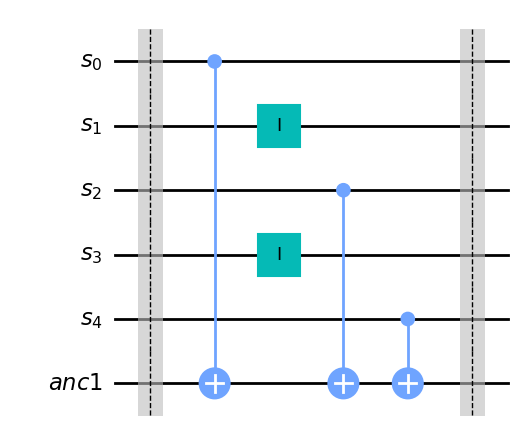
\includegraphics[width=\textwidth]{TFG/imagenes/BVgate2.png}
        \caption{Oráculo para la cadena $\mathbf{s}=10101$}
        \label{sFig:BVgate2}
    \end{subfigure}
        \caption{Ejemplo de oráculos para el algoritmo de BV}
    \label{FIG:BVOraculo}
 \end{figure}


 \textbf{Simulaciones}: Las simulaciones de este algoritmo ya han sido presentadas a lo largo del texto como ejemplo cuando se explicaban las distintas partes de la programación cuántica. Para ampliar estos ejemplos así como revisar el código, se pueden ver en el repositorio.\newline


\section{Simon}
\label{Sec3.5:Simon}
 El algoritmo de Simon, o de periodicidad de Simon, va a ser el primero que no va a usar únicamente computación cuántica, si no que la combina con computación clásica al final del mismo. Veremos cual es el problema y la parte cuántica de la solución, para así ver como procedemos posteriormente hasta encontrar la solución buscada. \newline

 Sea $f:\{0,1\}^{n} \rightarrow\{0,1\}^{n}$, la cual no conocemos su definición, pero si sabemos es periódica en el sentido de que existe una cadena binaria $\mathbf{c}=c_{0}c_{1}...c_{n-1}$ tal que $\forall \mathbf{x},\mathbf{y} \in \{0,1\}^{n}$ entonces, $f(\mathbf{x})=f(\mathbf{y})$ si y solo si $\mathbf{x}=\mathbf{y}\oplus\mathbf{c}$ , donde $\oplus$ es la suma binaria bit a bit. Llamaremos $\mathbf{c}$ al \textbf{periodo} de $f$. \newline

 \textbf{Problema}: Dada una función $f:\{0,1\}^{n} \rightarrow\{0,1\}^{n}$ con periodo $\mathbf{c}=c_{0}c_{1}...c_{n-1}$. Queremos determinar cual es el periodo de $f$ teniendo en cuenta que no conocemos su definición. \newline

 \textbf{Solución clásica}: Vamos ejecutando $f$ hasta encontrar una coincidencia. En el peor de los casos, la función es inyectiva y por lo tanto $\mathbf{c}=|\mathbf{0}\rangle$, para esto habrá que ejecutar $f$ al menos sobre la mitad del dominio, es decir, $2^{n-1}+1$ ejecuciones. Esto se debe a que si existiera un periodo distinto de \textbf{0}, ya habríamos encontrado alguna coincidencia entre la imagen de 2 elementos del dominio.  \newline
 
 Vamos a partir del circuito inicial, donde $U_{f}$ determina la función $f$:

 \vspace{10pt}

 \begin{center}$\Qcircuit @C=1.5em @R=1em {\lstick{|\mathbf{x}\rangle}& \qw {/^{n}} & \multigate{1}{U_{f}} & \qw {/^{n}} &\qw & \rstick{|\mathbf{x}\rangle}\\ \lstick{|\mathbf{y}\rangle} & \qw {/^{n}} &\ghost{U_{f}} & \qw {/^{n}} & \qw & \rstick{|\mathbf{y} \oplus f(\mathbf{x})\rangle}}$ \end{center}

 \vspace{7pt}

 \textbf{Algoritmo de Simon}, parte cuántica:

 \vspace{3pt}

 \begin{center}$\Qcircuit @C=1.5em @R=1em {
 \lstick{|\mathbf{0}\rangle}& \qw {/^{n}} & \gate{H^{\otimes n}} & \qw {/^{n}} & \multigate{1}{U_{f}} & \qw {/^{n}} & \gate{H^{\otimes n}} & \qw {/^{n}} & \meter & \qw \\ \lstick{|\mathbf{0}\rangle} & \dstick{\begin{matrix} \Uparrow \\ |\varphi_{0}\rangle \end{matrix}} \qw & \qw {/^{n}} & \dstick{\begin{matrix} \Uparrow \\ |\varphi_{1}\rangle \end{matrix}} \qw &\ghost{U_{f}} & \dstick{\begin{matrix} \Uparrow \\ |\varphi_{2}\rangle \end{matrix}} \qw & \qw {/^{n}} & \dstick{\begin{matrix} \Uparrow \\ |\varphi_{3}\rangle \end{matrix}} \qw  & \qw & \qw}$ \end{center}

 \vspace{30pt}

 Si lo observamos como operación matricial: $(H^{\otimes n}\otimes I)\:U_{f}\:(H^{\otimes n}\otimes I)\:|\mathbf{0},\mathbf{0}\rangle$\newline

 Análogamente al algoritmo de Deutsch-Jozsa, analizamos los estados del circuito:

 \begin{itemize}
     \item $\mathbf{|\varphi_{0}\rangle} = |\mathbf{0},\mathbf{0}\rangle$

    \vspace{5pt}

    \item  $\mathbf{|\varphi_{1}\rangle} = \dfrac{\sum_{\mathbf{x} \in \{0,1\}^{n}}|\mathbf{x},\mathbf{0}\rangle}{\sqrt{2^{n}}}$

    \vspace{5pt}

    \item $\mathbf{|\varphi_{2}\rangle} = \dfrac{\sum_{\mathbf{x} \in \{0,1\}^{n}}|\mathbf{x},f(\mathbf{x})\rangle}{\sqrt{2^{n}}}$

    \vspace{5pt}
    
    \item $\mathbf{|\varphi_{3}\rangle} =\dfrac{\sum_{\mathbf{x} \in \{0,1\}^{n}}\sum_{\mathbf{z} \in \{0,1\}^{n}}(-1)^{\langle \mathbf{z},\mathbf{x}\rangle}|\mathbf{z},f(\mathbf{x})\rangle}{2^{n}}$

 \end{itemize}

 Si bien antes era algo más directo que nos proporcionaba el resultado, aquí tenemos que analizarlo un poco más, ver hasta donde llega nuestro algoritmo cuántico y que es lo que obtenemos de él. La propiedad principal es la periodicidad de $f$, por lo que por definición  $|\mathbf{z},f(\mathbf{x})\rangle=|\mathbf{z},f(\mathbf{x}\oplus \mathbf{c})\rangle$. Vamos a estudiar el coeficiente al agruparlos, al ser mismo ket:

 \begin{equation}
    \begin{split}
     \dfrac{(-1)^{\langle \mathbf{z},\mathbf{x}\rangle}+(-1)^{\langle \mathbf{z},\mathbf{x}\oplus \mathbf{c}\rangle}}{2} &= \dfrac{(-1)^{\langle \mathbf{z},\mathbf{x}\rangle}+(-1)^{\langle \mathbf{z},\mathbf{x}\rangle \oplus \langle \mathbf{z}, \mathbf{c}\rangle}}{2} \\ &= \dfrac{(-1)^{\langle \mathbf{z},\mathbf{x}\rangle}+(-1)^{\langle \mathbf{z},\mathbf{x}\rangle}(-1)^{\langle \mathbf{z}, \mathbf{c}\rangle}}{2}
    \end{split}
 \end{equation}

 Por lo que si $\langle \mathbf{z}, \mathbf{c}\rangle=1$, entonces los sumandos se cancelan. Por otra parte, si $\langle \mathbf{z}, \mathbf{c}\rangle=0$ el coeficiente será $(\pm 1)$, es decir, al realizar la medición sobre el primer bloque de qubits, solo obtendremos aquellos tales que $\langle \mathbf{z}, \mathbf{c}\rangle=0$.

 \vspace{14pt}

 Pero, ¿proporciona esto una solución esto nuestro algoritmo? Visto así directamente puede parecer que no, debido a que cada vez que lo ejecutemos nos proporcionará una cadena distinta que tiene esa característica. Pero tras obtener n cadenas, obtenemos un sistema de ecuaciones a partir del cual obtenemos la cadena $\mathbf{c}$ deseada. Aquí es donde entraría la computación clásica para acabar de resolver el problema.

 \vspace{14pt}

 Se puede ver la mejora respecto a la solución clásica, ya que al ser todas las cadenas equiprobables, obtendremos $n$ cadenas distintas en menos ejecuciones que $2^{n-1}+1$, para $n$ suficientemente grande. Se puede ver un ejemplo concreto del desarrollo completo del algoritmo con $f:\{0,1\}^{3} \rightarrow\{0,1\}^{3}$ en \textit{Quantum computing for computer scientists, 190}\cite{B:QuantumScientist:2008}.

 \vspace{14pt}

 \textbf{Oráculo}: Debido a su complejidad se importa directamente desde Qiskit.\newline

 \textbf{Simulaciones}: Debido a que utilizamos este circuito, sin ninguna modificación, al comprobar nuestras MR, las simulaciones se encuentran en el \href{https://github.com/rodelanu/TFG/tree/main}{repositorio común}, en el archivo \href{https://github.com/rodelanu/TFG/blob/main/3_Simon_Rules.ipynb}{sobre las reglas del algoritmo de Simon}.

 \vspace{10pt}

 El circuito, análogo al teórico presentado anteriormente, para el algoritmo de Simon, con una cadena $\mathbf{c}$ de longitud 3 es:

 
 \begin{figure}[H]
    \centering
    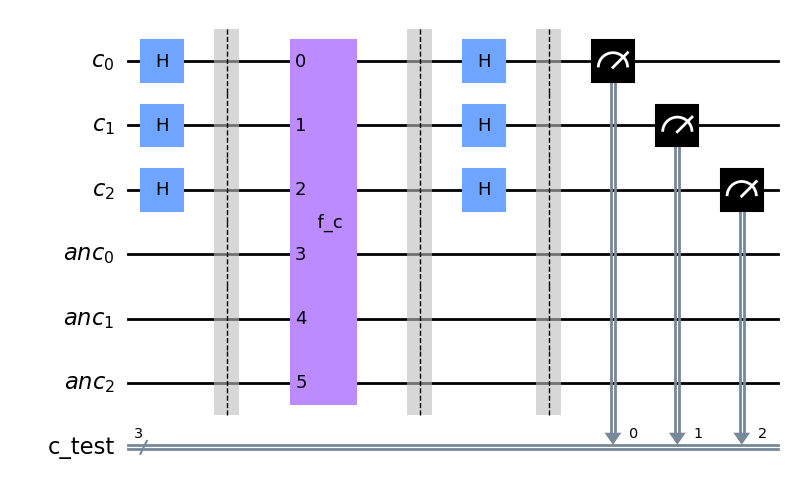
\includegraphics[width=0.7\textwidth]{TFG/imagenes/simon1.png}
    \caption{Circuito, algoritmo Simon con $\mathbf{c}=100$}
    \label{Fig:CircuitoSimon1}
 \end{figure}

 Lo hemos simulado y ejecutado en un sistema cuántico de IBM y estos son los resultados. Además de observar el ruido del sistema cuántico, se va a poder apreciar ambas formas de realizar el histograma, ya sea con conteo o probabilidades.

 \begin{figure}[H]
    \centering
    \begin{subfigure}[H]{0.48\textwidth}
        \centering
        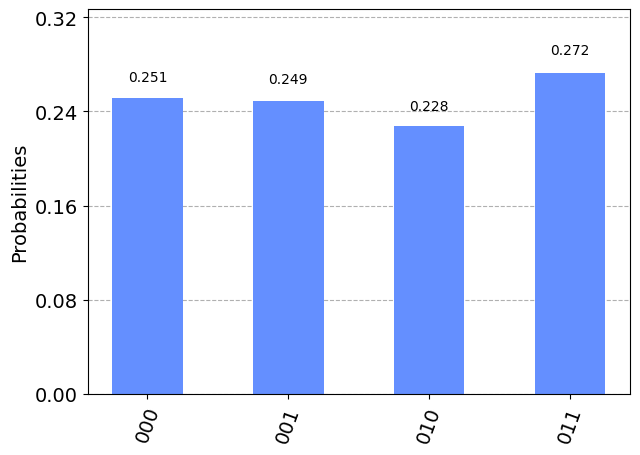
\includegraphics[width=\textwidth]{TFG/imagenes/simonSim.png}
        \caption{Simulador}
        \label{sFig:SimonSim}
    \end{subfigure}
    \hfill
    \begin{subfigure}[H]{0.48\textwidth}
        \centering
        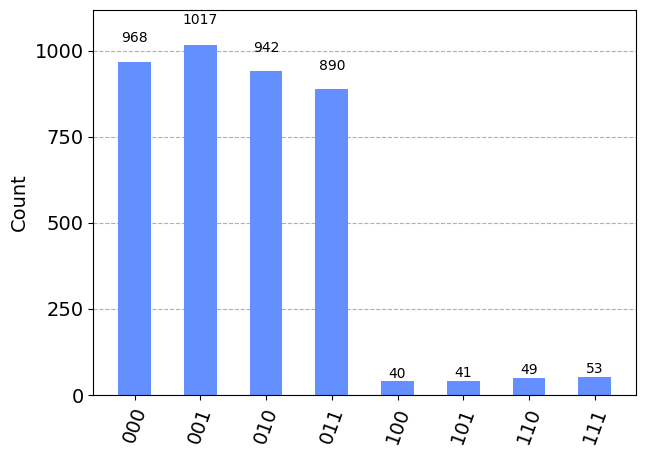
\includegraphics[width=\textwidth]{TFG/imagenes/simonReal.png}
        \caption{Sistema cuántico}
        \label{sFig:SimonIBM}
    \end{subfigure}
        \caption{Resultados del algoritmo Simon para la cadena $\mathbf{c}=100$. }
    \label{FIG:SimonRes}
 \end{figure}
    
\section{Transformada cuántica de Fourier}
\label{Sec3.6:Fourier}

Este apartado va a tratar sobre la transformada cuántica de Fourier, QFT del inglés \textit{Quantum Fourier transform} y una de sus aplicaciones más directas, la estimación cuántica de fase, QPE del inglés \textit{Quantum phase estimation}. Si bien es cierto que todos los algoritmos anteriores tenían un problema a resolver, el estudio de estos algoritmos se basan en la gran utilidad que tienen en cualquier contexto incluida la computación cuántica. Aunque en esta memoria no se tratarán algoritmos o técnicas que necesitan de estos materiales, podemos adelantar que dos de los algoritmos más importantes que se presentan actualmente en programación cuántica lo usan, como por ejemplo el algoritmo de Grover o de búsqueda y el algoritmo de Shor o de factorización.

\subsection{QFT}
Para introducir la transformada de Fourier vamos a ver como se comporta en el caso discreto, ya que nuestra versión cuántica partirá de aquí. 

\subsection{QPE}
 here